
% Tamoanchan Revisited chapter ----------------------------------------
\chapter*{Tamoanchan Revisited}
\addcontentsline{toc}{chapter}{Tamoanchan Revisited}

\begin{flushright}
\parbox{0.6\textwidth}{
\emph{I dream, therefore I exist. \\
\hspace*{\fill}{\textperiodcentered \textperiodcentered \textperiodcentered \hspace*{0.2em} August Strindberg} } }
\end{flushright}

\noindent
Tamoanchan Revisited is chess variant which is played on 22 x 22 board,
with bright cyan and blue fields and light green and dark blue pieces.
In algebraic notation, columns are enumerated from 'a' to 'v', and rows
are enumerated from '1' to '22'. A new piece is introduced, Serpent.

\clearpage % ..........................................................

\section*{Serpent}
\addcontentsline{toc}{section}{Serpent}

\noindent
\begin{wrapfigure}{l}{0.4\textwidth}
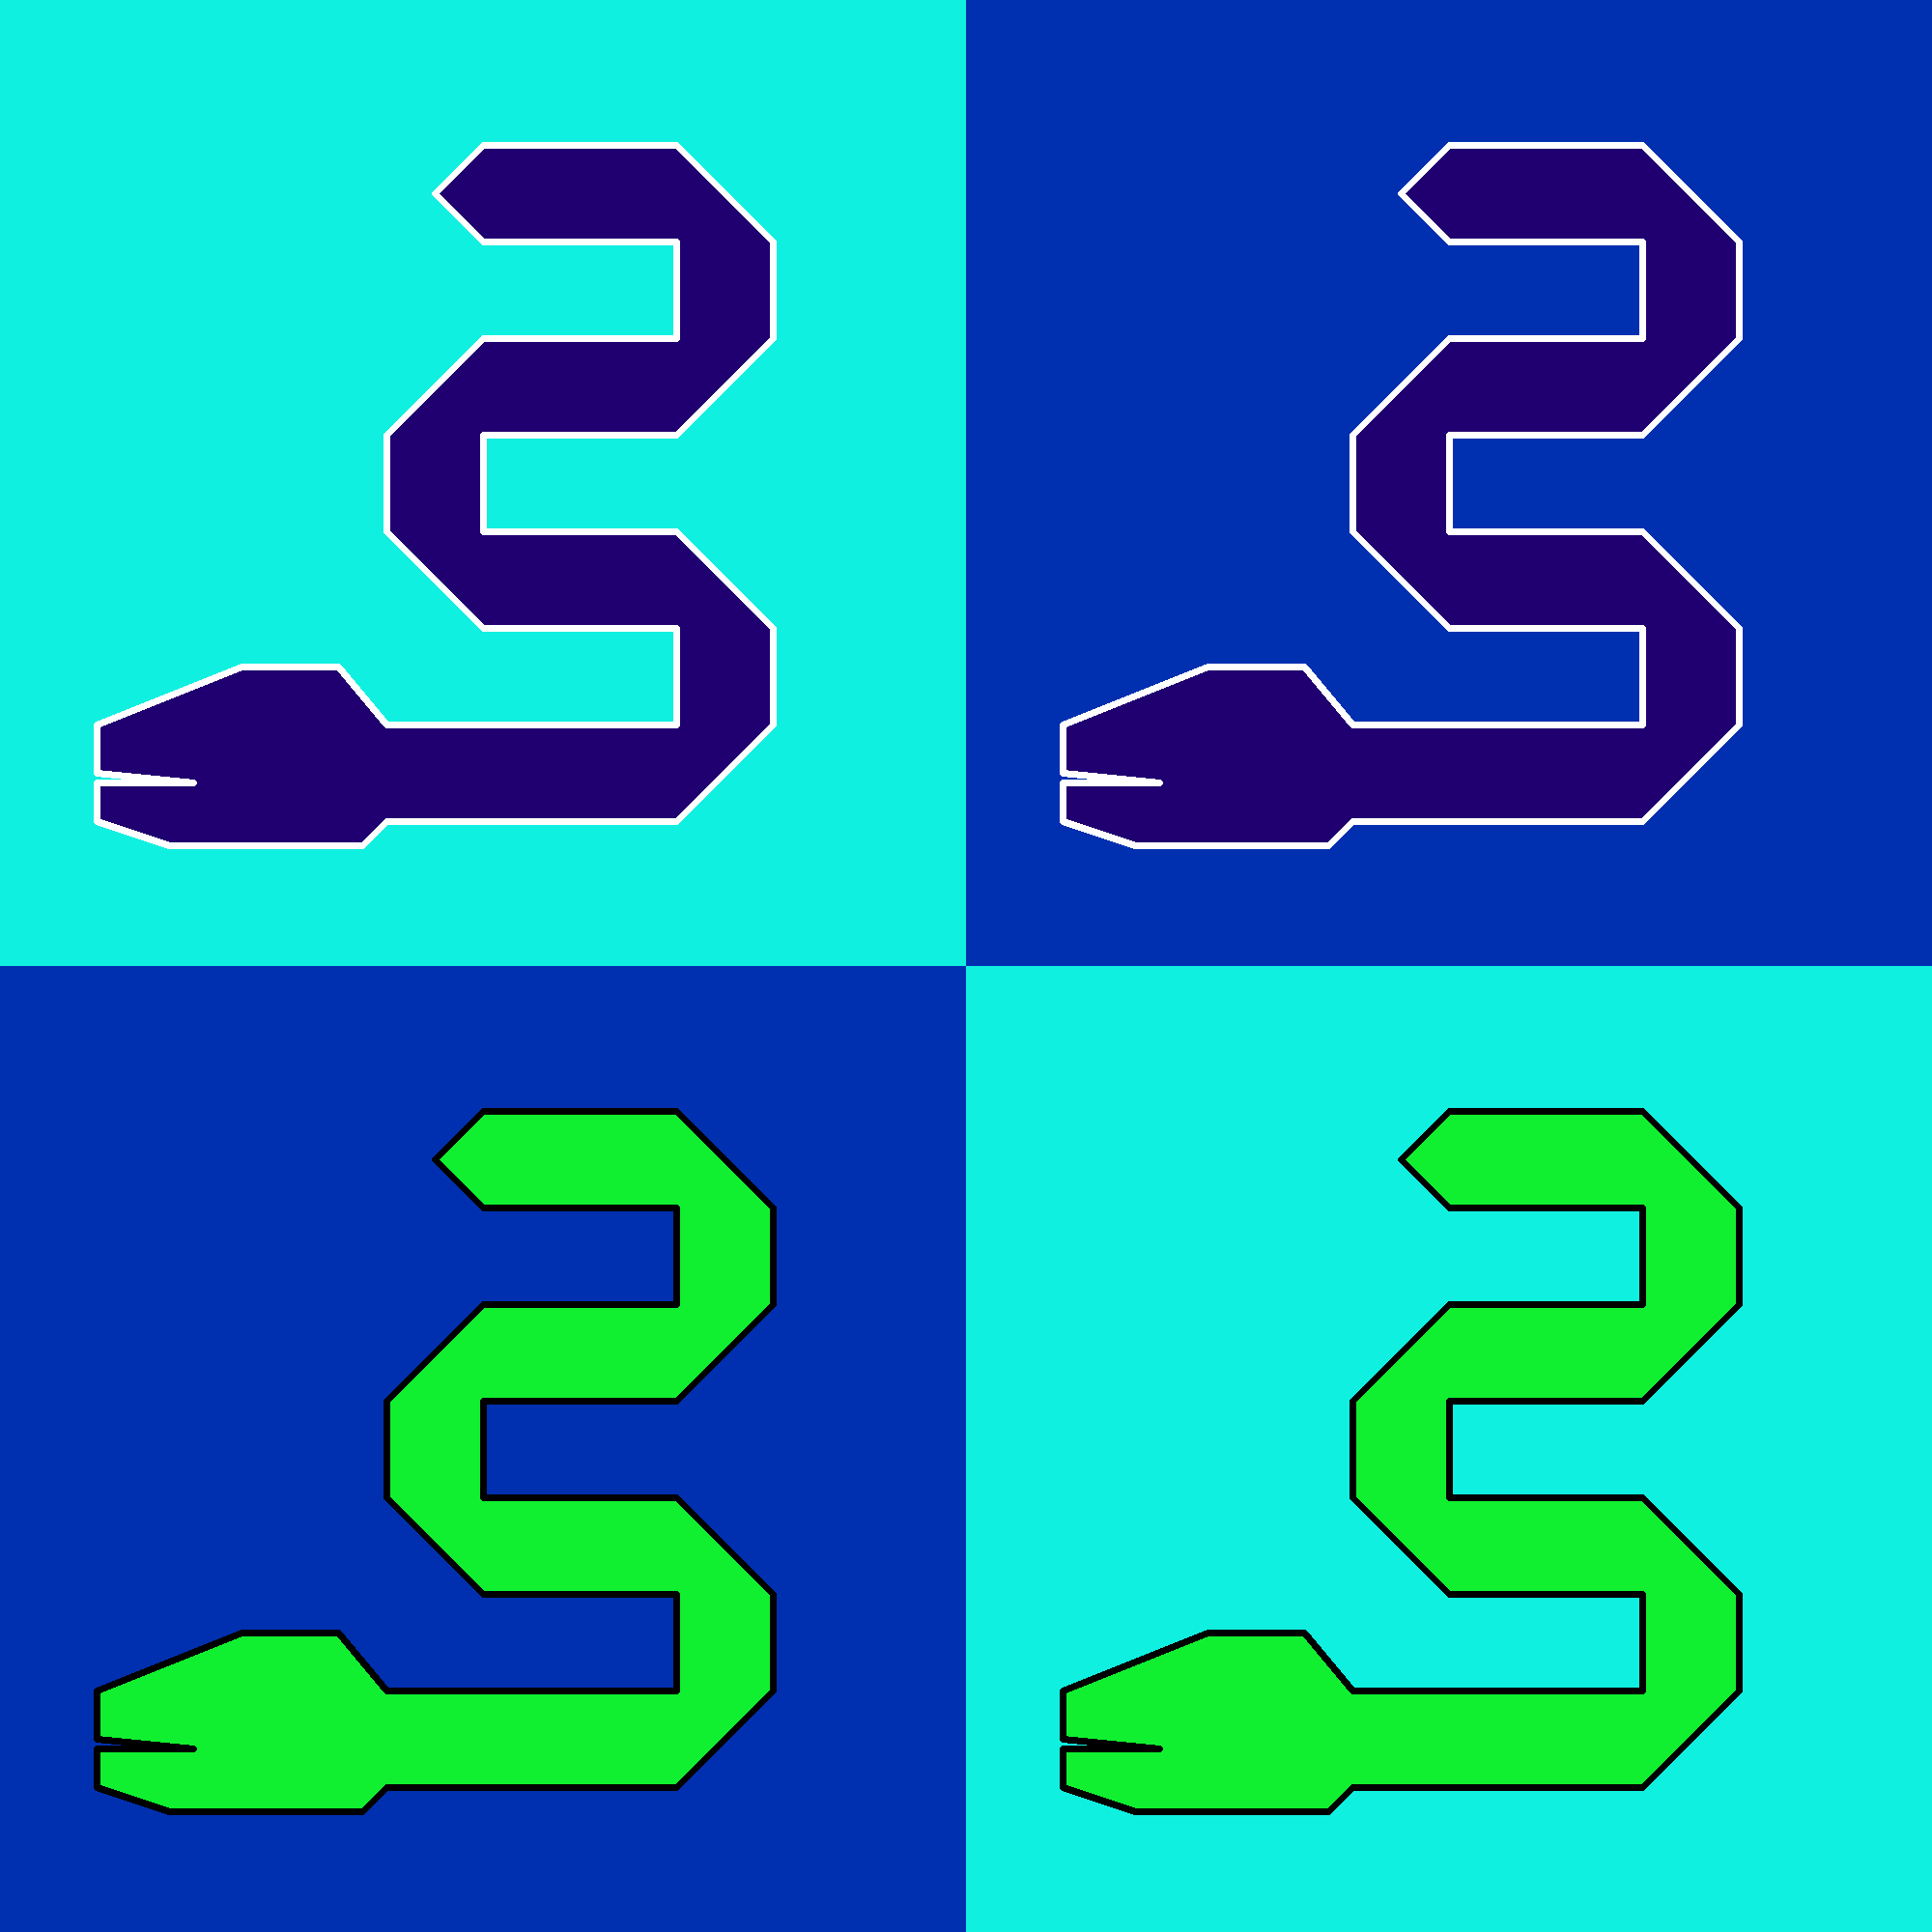
\includegraphics[width=0.4\textwidth, keepaspectratio=true]{pieces/13_serpent.png}
\caption{Serpent}
\label{fig:13_serpent}
% % \centering
\end{wrapfigure}

\clearpage % ..........................................................

\section*{Initial setup}
\addcontentsline{toc}{section}{Initial setup}

Initial setup can be seen in image below:

\noindent
% \begin{figure}[t]
\begin{figure}[h]
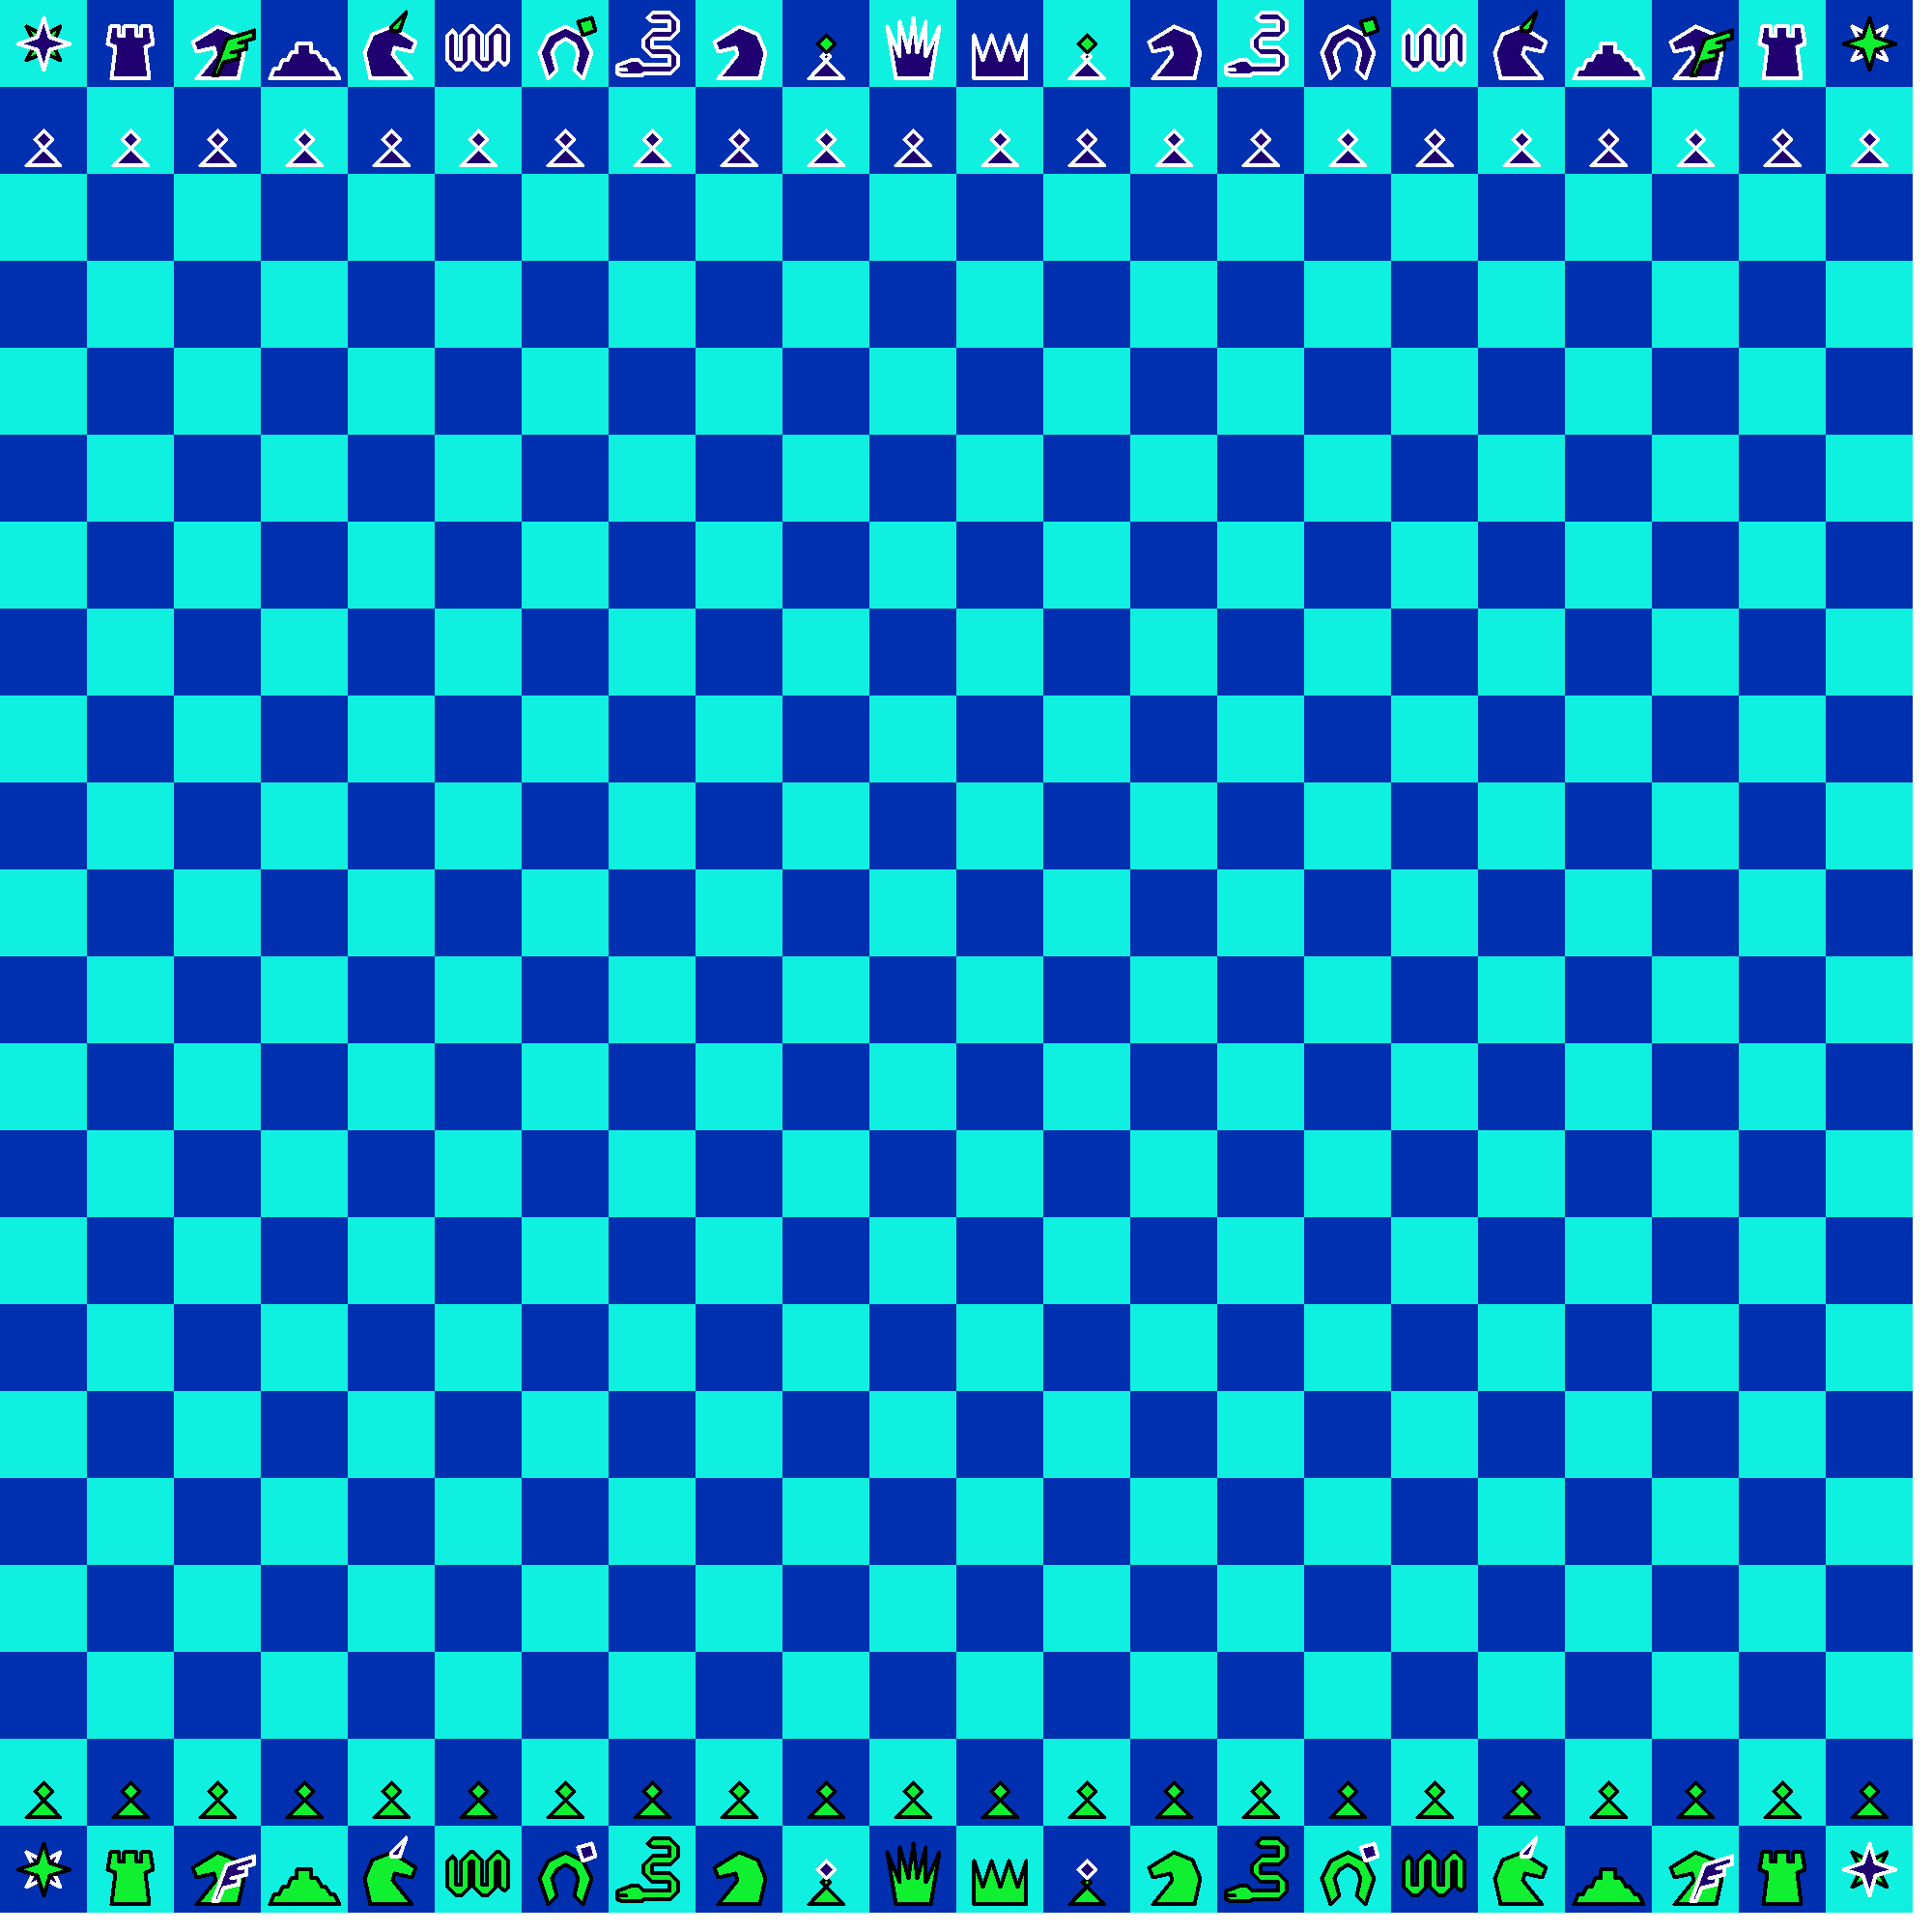
\includegraphics[width=1.0\textwidth, keepaspectratio=true]{boards/16_tamoanchan_revisited.png}
\caption{Tamoanchan Revisited board}
\label{fig:16_tamoanchan_revisited}
% \centering
\end{figure}

\clearpage % ..........................................................
% ---------------------------------------- Tamoanchan Revisited chapter
